\chapter{הבית החכם והאינטרנט של הדברים}

\begin{epigraph}{}
פעם נעלנו את הדלת כדי שאיש לא יידע מה קורה בפנים. היום הדלת עצמה יודעת, ומדווחת.
\end{epigraph}

\section{הבית שמקשיב}

במשך עשרות אלפי שנים, הבית היה המקום שבו מסתתרים מהעולם. מערה, אוהל, בקתה, דירה. קירות עבים, דלת נעולה, ובפנים פרטיות. ההיסטוריה של האדריכלות היא במידה רבה היסטוריה של הפרדה בין "בפנים" לבין "בחוץ".

הבית החכם מטשטש את הגבול הזה. הנורה נדלקת כשאתם נכנסים. התרמוסטט לומד באיזו שעה אתם חוזרים מהעבודה. הרמקול בסלון מחכה למילת ההפעלה, ובשביל זה הוא צריך להקשיב כל הזמן. המקרר יודע מתי נגמר החלב, והשואב הרובוטי מכיר את מפת הדירה טוב יותר מהאורחים.

כל זה נכנס תחת שם כללי: \textbf{האינטרנט של הדברים} (\en{Internet of Things}, או \en{IoT}). הרעיון פשוט. לא רק אנשים מתחברים לרשת, אלא גם חפצים. והחפצים, בניגוד לאנשים, לא ישנים אף פעם.

\begin{figure}[!htb]\centering
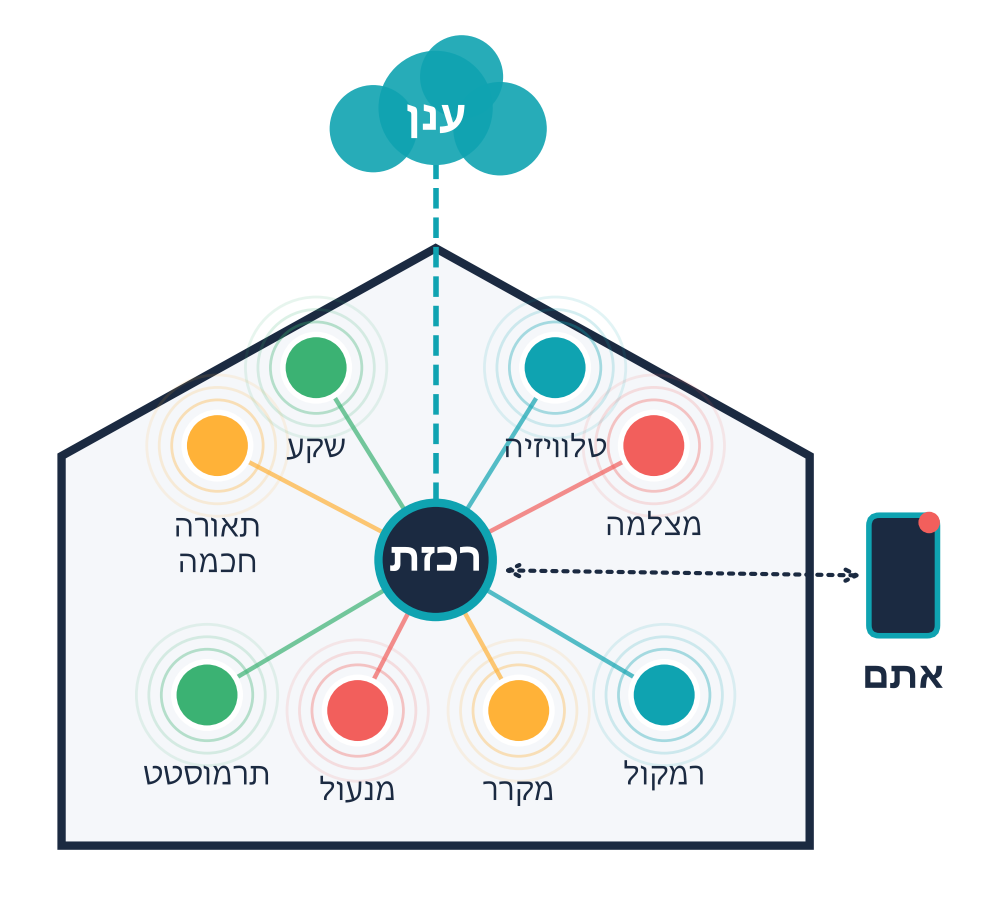
\includegraphics[width=0.85\textwidth]{images/smart_home.png}
\caption[הבית החכם: מכשירים מחוברים לרשת]{הבית החכם: מכשירים יומיומיים שמחוברים לרשת ומתקשרים זה עם זה ועם הענן. האיור נוצר ב-\en{Python}.}\label{fig:smart-home}\end{figure}

איור~\ref{fig:smart-home} ממחיש את הרעיון. כל מכשיר בבית הוא צומת ברשת. כל אחד מהם אוסף מידע קטן ותמים לכאורה: טמפרטורה, תנועה, צריכת חשמל, קול. אבל כשמחברים את כל הנקודות, מתקבלת תמונה מפורטת להפתיע של החיים בתוך הבית.

\section{יותר משמונה-עשר מיליארד חפצים מחוברים}

כמה "דברים" כבר מחוברים? לפי חברת המחקר \en{IoT Analytics}, ב-\num{2024} היו בעולם כ-\num{18.5} מיליארד מכשירים מחוברים. בדוח שפרסמה באוקטובר \num{2025} היא חזתה כ-\num{21.1} מיליארד עד סוף \num{2025} \parencite{iotanalytics2025}. כלומר, \num{18.5} הוא הנתון המדוד האחרון בדוח, ו-\num{21.1} הוא תחזית שפורסמה לפני סוף השנה, לא מדידה. צריך לקרוא את המספר הזה בזהירות. רובם המכריע של המכשירים האלה אינם בבתים: המספר כולל גם חיישנים במפעלים, בחקלאות ובתחבורה. לכן הוא איננו מודד בתים חכמים, ואין טעם להעמיד אותו מול מספר בני האדם המחוברים. מה שהוא כן מראה הוא שהרשת כבר איננה רק רשת של בני אדם.

\begin{factbox}[מכשירים מחוברים בעולם]
\begin{itemize}
  \item 2022: כ-14.4 מיליארד
  \item 2023: כ-16.7 מיליארד
  \item 2024: כ-18.5 מיליארד
  \item 2025: כ-21.1 מיליארד (תחזית מאוקטובר \num{2025})
  \item 2030: כ-39 מיליארד (תחזית מאוקטובר \num{2025})
\end{itemize}
מקור: \textcite{iotanalytics2025}. כל המכשירים המחוברים בעולם, לא רק בבתים.
\end{factbox}

הסדרה הזאת מראה האצה. בין 2022 ל-2024 נוספו כארבעה מיליארד מכשירים בתוך שנתיים. אם תחזית \num{2025}, שפורסמה באוקטובר של אותה שנה, התממשה, הרי שבתוך שלוש שנים בלבד נוספו כשבעה מיליארד מכשירים, ולפי התחזית, עד 2030 המספר יגדל פי שניים ויותר לעומת 2024 \parencite{iotanalytics2025}. אלה תחזיות של חברת מחקר, לא מדידות, והן כוללות את כל המכשירים המחוברים, לא רק את אלה שבבית. הרשת, שהתחילה כקשר בין כמה מחשבים באוניברסיטאות, הופכת למערכת עצבים שעוטפת את כדור הארץ.

\section{נוחות במחיר פרטיות}

למה בכלל להכניס את כל זה הביתה? כי זה נוח, ולעיתים אפילו מציל חיים. חיישן עשן ששולח התראה לטלפון כשאתם רחוקים. מנעול שנפתח לילד ששכח מפתח. מערכת שמזכירה לקשיש ליטול תרופה. מזגן שנכבה כשאיש לא בבית וחוסך חשמל. אין כאן רק שעשועים. יש כאן שירותים אמיתיים.

אבל לכל נוחות יש מחיר, והמחיר כאן הוא מידע. מי שיודע מתי האורות כבים יודע מתי אתם ישנים. מי שיודע מתי הדלת נפתחת יודע מתי הבית ריק. ומי שמקשיב לסלון, גם אם רק לצורך זיהוי מילת הפעלה, נמצא קרוב מאוד לשיחות הפרטיות ביותר שלכם.

זוכרים את מעגל כלכלת הקשב מפרק~\ref{ch:attention}? שושנה זובוף תיארה כיצד החוויה האנושית הופכת לחומר גלם לנתוני התנהגות \parencite{zuboff2019}. הבית החכם מרחיב את המכרה הזה אל המקום האינטימי ביותר שיש. אם הסמארטפון יודע מה אתם עושים בחוץ, הבית החכם יודע מה אתם עושים בפנים.

\begin{alertbox}[שאלות לפני שמחברים מכשיר חדש]
\begin{itemize}
  \item איזה מידע המכשיר אוסף, והאם הוא באמת צריך אותו כדי לעבוד?
  \item לאן המידע נשלח, ולכמה זמן הוא נשמר?
  \item האם אפשר לכבות את המיקרופון או את המצלמה בלחיצה פיזית?
  \item מה יקרה למכשיר, ולמידע, אם החברה שמאחוריו תיסגר או תימכר?
\end{itemize}
\end{alertbox}

\section{מי הבעלים של המטבח שלכם?}

יש כאן גם שאלה עמוקה יותר, שקשורה לבעלות. במשך רוב ההיסטוריה, כשקניתם כיסא, הכיסא היה שלכם. אף אחד לא יכול היה לשנות אותו מרחוק. היום, מכשיר חכם הוא במידה רבה שירות. החברה יכולה לעדכן אותו, לשנות את התנאים, להוסיף פרסומות, או להפסיק לתמוך בו. ייתכן שקניתם את הקופסה, אבל לא את מה שמתרחש בתוכה.

ויש גם צד ביטחוני. כל מכשיר מחובר הוא דלת נוספת אל הרשת הביתית. מצלמה זולה עם סיסמת ברירת מחדל, נורה שלא קיבלה עדכון אבטחה כבר שנים, או צעצוע שמדבר עם הענן, עלולים להפוך לנקודת תורפה. בעולם הישן, פורץ היה צריך לשבור חלון. בעולם החדש, לפעמים מספיק לו שמישהו שכח לשנות סיסמה.

ובכל זאת, אם להסתכל לאחור במבט רחב, נדמה שטכנולוגיות ביתיות חדשות רבות עוררו בהתחלה חשד. החשמל נראה מסוכן, הטלפון נראה פולשני, והטלוויזיה נראתה כמו אורח שלא הולך הביתה. עם הזמן פיתחו החברות האנושיות כללים, תקנים וחוקים שהפכו כל אחת מהטכנולוגיות האלה לבטוחה יותר. סביר להניח שזה יקרה גם עם הבית החכם. השאלה היא כמה מידע נאבד בדרך, עד שהכללים יתעדכנו.

זה לא אומר שצריך לחזור לנרות ולמפתחות ברזל. זה אומר שהשאלה "האם זה נוח?" צריכה לבוא יחד עם שאלה נוספת: "מי עוד נהנה מהנוחות שלי?".

\begin{thinkbox}
דמיינו שכל המידע שנאסף בבית שלכם במשך שנה מודפס בספר אחד. האם הייתם מסכימים שזר יקרא אותו? ואם לא, למה אתם מסכימים שמחשב של זר יקרא אותו?
\end{thinkbox}
